\documentclass[a4paper,12pt]{report}

\usepackage[brazil]{babel}
\usepackage[utf8]{inputenc}
\usepackage[T1]{fontenc}
\usepackage{listings}
\usepackage{color}
\usepackage{graphicx}

\usepackage[top=2cm,bottom=2.5cm,left=2.5cm,right=2cm]{geometry}
\lstset{basicstyle=\small,breaklines=true,frame=single,numbers=left}

\begin{document}

    \begin{titlepage}
        \begin{center}

            % \large
            UNIVERSIDADE DE SÃO PAULO\\
            Escola Politécnica\\
            Departamento de Computação e Sistemas Digitais
            \vspace{8cm}
            
            \Huge
            \textbf{Compilador Allegri}
            
            \vspace{0.5cm}
            \large
            Projeto Final da Disciplina de Compiladores - PCS 2508
            
            \vspace{2.5cm}
            \Large
            Gabriel Casarin da Silva
            
        \end{center}
        
        \vspace{3.0cm}
        \setlength{\parindent}{10.5cm}
        \large Professor Responsável:

        \setlength{\parindent}{10.5cm}
        Prof. Dr. João José Neto
        

        \begin{center}
            \vfill
            \large
            São Paulo, 2016
        \end{center}
            
    \end{titlepage}
        

    \tableofcontents
    % \renewcommand{\labelitemi}{\textendash}
    \newpage
    \chapter*{Introito}
    \addcontentsline{toc}{part}{Introito}
    O projeto da disciplina PCS 2508 - Linguagens e Compiladores de 2016 consistiu em desenvolver uma linguagem de programação e projetar um compilador para ela. A linguagem desenvolvida foi denominada Barber. O seu compilador, Allegri.

    Por isso, este documento é divido em duas partes. A primeira descreve a linguagem Barber, sua motivação e aspéctos teóricos. A segunda documenta as etapas do desenvolvimento do compilador Allegri.

    Ao final, trazemos uma série de programas-exemplo e de testes dos códigos de máquina gerados pela compilação \textemdash ~ testes estes realizados no simulador de Máquina de von Neumann (MVN).
    
    \addcontentsline{toc}{part}{Um Prelúdio à Linguagem Barber}
    \part*{Um Prelúdio à Linguagem Barber}

    \addcontentsline{toc}{section}{Motivação}
    \section*{Motivação}
    O desafio de se criar uma nova linguagem de programação está no compromisso que deve ser feito entre os recursos que essa linguagem deve suportar, a complexidade de sua sintaxe, o propósito de utilização, o suporte a um ou vários tipos de hardware, eficiência no desenvolvimento de software, legibilidade do código, etc.

    Além disso, deve-se escolher o paradigma (ou paradigmas) que essa linguagem deverá seguir. Um dos paradigmas que obteve grande sucesso desde o seu surgimento é o Paradigma Estrurado. Ele surgiu como reação à necessidade de se desenvolver código com correição, re-utilizável e portável. O projeto de um compilador de uma linguagem estruturada pode ser feito de maneira simplificada, uma vez que há entre a maioria dos comandos daquela e o código de máquina que os implementa traduções diretas.  

    Das linguagens não interpretadas de propósito geral, apenas duas continuam a ser usadas extensivamente \textemdash ~ C e C++. C vem da época dos primeiros computadores mono-usuário. Sua sintaxe soa antiquada e o processo de depuração demasiado complexo para as necessidades de desenvolvimento ágil atual. Mesmo assim, ela ainda é utilizada para desenvolvimento de software embarcado e de sistemas operacionais. C++ continua sendo desenvolvida, porém sua sintaxe complexa implica em compilação ineficiente e demorada. Além disso, sua curva de aprendizado é íngreme e impõe obstáculos ao desenvolvimento de grandes projetos de software.

    Nesse contexto surgiu a linguagem Go. Seu objetivo é ser uma linguagem compilada (tal como C e C++), ter uma sintaxe simplificada e ao mesmo tempo trazer suporte às novas tendências da Computação. Por isso, o processo de desenvolvimento em Go é ágil e sua compilação, eficiente.

    A linguagem Barber buscou inspirar-se na filosofia que deu origem à linguagem Go. A linguagem aqui apresentada pretende ser didática, ter uma sintaxe compacta, facilmente extensível, regular e de fácil aprendizado, permitir o desenvolvimento ágil e ter um código legível. O seu compilador, Allegri, foi projetado para gerar código assembly para uma Máquina de von Neumann genérica (MVN).

    \newpage
    \section*{Sintaxe}
    \addcontentsline{toc}{section}{Sintaxe}
    A sintaxe é especificada usando a notação de Wirth:
    \begin{lstlisting}[numbers=none,frame=none]
    DefineFunc       =  "def" Identificador [Tipo] "enter"
                        { DeclaraParam } Bloco .

    DeclaraParametro =  "par" Identificador {, Identificador}
                              Tipo {"[" "]"}.

    DeclaraVariavel  =  "var" Identificador {"," Identificador}
                              Tipo { "[" Numero "]" } .

    Bloco            =  "{" {"enter" [Comando]} "}".

    Comando          =  (DeclaraVariavel
                        | Atribuicao
                        | Return
                        | IF
                        | WHILE
                        ) "enter" {"enter"} .

    IF               =  "if" Teste Bloco
                            { "elif" Teste Bloco }
                            [ "else" Bloco ] .

    WHILE            =  "while" Teste Bloco .

    ConstBool        =  "True" | "False" .

    ExpressaoBool    =  TermoBool { "or" TermoBool } .

    TermoBool        =  FatorBool { "and" FatorBool }.

    FatorBool        =  ConstBool
                        | "not" FatorBool
                        | Operando
                        | "(" ExpressaoBool ")" .

    Expressao        =  ["-"] Termo { ("+" | "-") Termo } .

    Termo            =  Fator { ("*" | "/") Fator } .

    Fator            =  Numero
                        | Operando
                        | "(" Expressao ")" .

    Operando         =  Identificador [
                          "[" Expressao { "," Expressao } "]"
                          | "(" Expressao { "," Expressao } ")"
                        ] .

    Atribuicao       =  Operando "=" (Expressao | ExpressaoBool) .

    Return           =  "return" (Expressao | ExpressaoBool) .

    Comparacao       =  Expressao (
                            ">" | ">=" | "<"| "<=" | "=="| "!="
                        ) Expressao .

    Teste            =  Comparacao | ExpressaoBool .

    Tipo             =  "int"
                        | "char"
                        | "bool" .

    Identificador    =  ("Letra" | "_" )
                        {"Letra" | "Algarismo" | "_"} .

    Numero          =  "Algarismo" {"Algarismo"} .
    \end{lstlisting}

    \subsubsection*{Declaração de Função}
    \addcontentsline{toc}{subsection}{Declaração de Função}
    Uma declaração de função associa um identificador a uma função. Aquela deve ser iniciada com um \textbf{def} seguido de um nome. Caso ela retorne algum valor, deve indicar o tipo de valor que retorna. Caso for um procedimento, não é necessário declarar retorno de tipo \textit{void}. Nas próximas linhas, deve-se declarar os eventuais parâmetros formais que a função dependerá.

    Exemplo de declaração de função:

    \begin{lstlisting}[caption={Declaração de função}]
    def min int
        par x, y int {
        if x < y {
            return x
        }
        return y
    }
    \end{lstlisting}

    \subsubsection*{Declaração de Parâmetros Formais}
    \addcontentsline{toc}{subsection}{Declaração de Parâmetros Formais}
    Uma declaração de parâmetro simples segue a seguinte sintaxe:

    \begin{verbatim}
    DeclaraParametro =  "par" Identificador {, Identificador} Tipo {"[" "]"}. \end{verbatim}
    Tipo pode ser \textbf{int, char} ou \textbf{bool}. Caso o parâmetro seja uma referência a um vetor ou matriz, deve-se seguir o tipo com pares de abre-fecha colchete tantos quantos for o \textit{rank} do objeto (1 para vetor, 2 para matriz).

    Parâmetros formais são declarados logo abaixo da assinatura da função.
    
    \textit{Exemplo 1} ~
     No Listing 1, na linha 2, foram declarados dois parâmetros simples, x e y, de tipo \textbf{int}.

    \textit{Exemplo 2} ~
     Declaração de parâmetro vetor: ~~~\verb|par v int[]|
    
    \textit{Exemplo 3} ~
     Declaração de parâmetro matriz: ~\verb|par m int[][]|

    \subsubsection*{Declaração de Variáveis}
    \addcontentsline{toc}{subsection}{Declaração de Variáveis}
    Uma declaração de variável simples segue a seguinte sintaxe:
    \begin{verbatim}
DeclaraVariavel = "var" Identificador {"," Identificador} Tipo {"[" Numero "]"}. \end{verbatim}
    As declarações de variáveis são muito similares às de parâmetros formais, com exceção de que: (\textit{i}) elas devem ocorrer logo no início do bloco da função, entre o fim da declaração de parâmetros e o início do código; (\textit{ii}) as dimensões de vetores e matrizes precisam ser declarados como números constantes (não há suporte a alocação dinâmica).
    
    \textit{Exemplo 1} ~
     Declarações de variáveis simples são idênticas às de parâmetros formais, apenas com a palavra \textbf{par} trocada por \textbf{var}.

    \textit{Exemplo 2} ~
     Declaração de vetor: ~~~\verb|var v int[10]|
    
    \textit{Exemplo 3} ~
     Declaração de matriz: ~\verb|var m int[5][20]|


    \subsubsection*{Comandos condicionais}
    \addcontentsline{toc}{subsection}{Comandos condicionais}
    Os comandos condicionais são formados por blocos de cláusulas if-elif-else:

    \begin{lstlisting}
    if Condicao_1 {
        .
        .
        .
    }
    elif Condicao_2 {
        .
        .
        .
    }
    elif Condicao_3 {
        .
        .
        .
    }
    .
    .
    .
    else {
        .
        .
        .
    }
    \end{lstlisting}

    Esse comando executa o bloco da primeira condição satisfeita. Caso contrário, executa o bloco else.

    Não são necessários parênteses ao redor das condições.\\

    \textit{Exemplo} ~ O Listing 1 traz um exemplo de uma cláusula if única.


    \subsubsection*{Comando while}
    \addcontentsline{toc}{subsection}{Comando while}
    O comando \textbf{while} implementa laços de um programa. Sua sintaxe é extremamente simples:
    \begin{verbatim}
    WHILE = "while" Teste Bloco . \end{verbatim}
    Tal comando executa o que estiver dentro de Bloco até que a condição Teste reste falsa.
    \begin{lstlisting}
        i = 0
        while i < 10 {
            .
            .
            .
            i = i + 1
        }
    \end{lstlisting}

    % \newpage
    \section*{Como Compilar}
    \addcontentsline{toc}{section}{Como Compilar}
    A estrutura de diretórios do repositório do compilador é como segue:
    \begin{verbatim}
    ./Allegri
    |--- Barber Lang
    |--- comum
    |    +--- automatos
    |--- Meta Compilador
    |--- mvn_build_system
    |    |--- biblioteca
    |    |--- bin
    |    +--- src
    |--- src
    +--- util
    \end{verbatim}

    Diferentemente de outros compiladores, o arquivo com o código-fonte deve ser colocado em um diretório específico \textemdash \space ./Allegri/src \textemdash \space para ser compilado. Para compilar um arquivo \verb|foo.barber|, digite no terminal o seguinte comando:

    \begin{verbatim}
    $ make fonte=foo \end{verbatim}

    Caso o comando acima resulte em sucesso na compilação, o código assembly gerado é posto na pasta mvn\_build\_system/src sob o nome de \verb|foo.asm|. Nesse momento, o programa estará pronto para ser montado e, em seguida, executado na MVN.

    \section*{Ambiente de Execução MVN}
    \addcontentsline{toc}{section}{Ambiente de Execução MVN}
    Após o processo de compilação, faz-se necessária ainda a montagem do código assembly. O montador, linkador e a própria MVN foram obtidos de disciplinas anteriores.
    A máquina em que vamos simular os programas compilados é bem limitada no seu conjunto de instruções. Por isso, tomamos a liberdade de escrever uma pequena biblioteca de sub-rotinas auxiliares, as quais implementam para a MVN as funcionalidades de:
    
    \begin{enumerate}
        \item Operações com tipos booleanos (and, or e not), comparações entre valores, etc.;
        \item Definir o valor das constantes True e False, além de reservar espaço para registradores especiais como FP (\textit{frame pointer}), SP (\textit{stack pointer}) e ACC\_AUX (acumulador auxiliar);
        \item Instruções para leitura e escrita em endereços e relativos tanto a:
            \begin{enumerate}
                \item o \textit{frame pointer} \textemdash~ utilizado para variáveis e parâmetros;
                \item endereços absolutos da área de dados (pointeiros) \textemdash~ utilizado para indexação de vetores e matrizes;
            \end{enumerate}
        \item Alocação de espaço estático na área de dados;
        \item Comandos de Push e Pop na pilha de execução do programa;
    \end{enumerate}

    Eis a estrutura do Ambiente de Execução MVN:
    \begin{verbatim}
    ./mvn_build_system
    |-- biblioteca
    |   |-- boolean.asm
    |   |-- boolean_op.asm
    |   |-- comparacao.asm
    |   |-- const.asm
    |   |-- environment.asm
    |   |-- heap.asm
    |   +-- push_pop.asm
    |-- bin
    |   |-- MLR.jar
    |   |-- mvn.jar
    |   +-- saida.mvn
    |-- Makefile
    |-- saida.mvn -> bin/saida.mvn
    +-- src
    \end{verbatim}

    Quando o comando \verb|make| é executado para compilar um código-fonte, ele automaticamente chama o montador da MVN, depois o seu linkador (para ligar o código compilado com a biblioteca do ambiente de execução) e passa a executar o código pronto. O código de máquina resultante da linkagem é salvo no arquivo ./bin/saida.mvn. Caso se queira apenas executar o montador para o arquivo \verb|bar.asm|, deve-se executar no terminal o seguinte comando:

    \begin{verbatim}
    $ make bar \end{verbatim}

    E para iniciar o simulador MVN,

    \begin{verbatim}
    $ make run \end{verbatim}



    \part*{Compilador Allegri\\\textit{Da capo}}
    \addcontentsline{toc}{part}{Compilador Allegri - Da capo}

    %%%%%%%%%%%%%%%%%%%%%%%%
    %      ARQUITETURA     %
    %%%%%%%%%%%%%%%%%%%%%%%%

    \chapter*{Arquitetura}
    \addcontentsline{toc}{section}{Arquitetura}
    O compilador compõe-se de duas partes: o Front End (analisadores léxico e sintático) e o Gerador de Código Assembly (analisador semântico). O Back End para a geração de código de máquina fica a cargo do montador da MVN.

    A arquitetura básica do compilador é dada pela figura a seguir\footnote{Obs: não há otimização de código como sugere a figura.}: 

    % \begin{figure}[h]
    %     \centering
    %     \caption{}
    %     \includegraphics[scale=1]{}
    % \end{figure}

    \begin{figure}[h]
        \caption{Arquitetura do compilador}
        \centering
        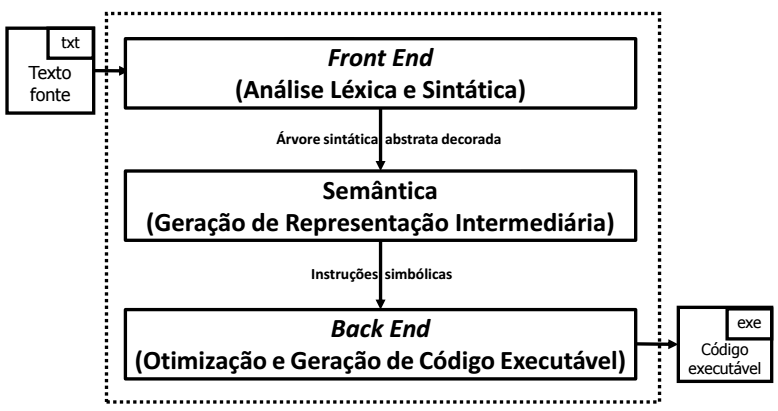
\includegraphics[scale=.5]{esqueleto}
    \end{figure}

    Toda a atividade do compilador Allegri orbita o Analisador Sintático. Compiladores que têm o Analisador Léxico como rotina principal são ditos seguir o paradigma de \textit{syntax driven compilation}. Em tais compiladores, os analisadores Léxico e Semântico (dentre outros sub-módulos necessários) são sub-rotinas acionadas por aquele. Isso significa que a atividade de análise léxica é desempenhada apenas nos momentos em que o Analisador Sintático solicitar.

    Ora, a arquitetura escolhida para cada componente do compilador é a de Motor Dirigido por Eventos. Nessa visão, cada sub-rotina reage a certos estímulos, cujos tratamentos alteram o estado do motor e gera saídas condicionadas ao pé da análise. Por exemplo, a sub-rotina de decomposição de texto-fonte deve reagir ao evento de chegada de nova linha. E o Analisador Léxico, ao de chegada de novo caractere, etc.

    Nas próximas seções especificamos o projeto e implementação de cada módulo do compilador.

    %%%%%%%%%%%%%%%%%%%%%%%%%%%
    %      ANÁLISE LÉXICA     %
    %%%%%%%%%%%%%%%%%%%%%%%%%%%

    \chapter*{Análise Léxica}
    \addcontentsline{toc}{section}{Análise Léxica}
    O analisador léxico é um dispositivo que - dada linguagem de programação - extrai átomos de um texto-fonte.

    Ele se baseia em uma gramática léxica derivada da gramática principal da linguagem. Seu princípio de funcionamento é o de um autômato finito transdutor. Ele pode operar certas funções semânticas, bem como filtrar tabulações, espaços em branco e comentários.

    No meu projeto, decidi fazer um dispositivo que desempenhasse o seu papel de acordo com as especificações dadas em um autômato finito fornecido à parte, nos moldes daqueles desenvolvidos na disciplina de Lógica Computacional.

    \subsection*{Gramática Léxica}
    \addcontentsline{toc}{subsection}{Gramática Léxica}
    A gramática léxica descreve como os caracteres sequenciados a partir do texto-fonte devem ser aglutinados a fim de que tais aglutinações possam ser devidamente fornecidas ao analisador sintático.
    
    Na linguagem Barber, os tokens devem obedecer às seguintes formas:

    \begin{lstlisting}
    Identificador = ("Letra" | "_") {"Letra" | "Algarismo" | "_"} .
    CifraDecimal  = "Algarismo" {"Algarismo"} .
    CifraHexadec  = "0x" {CifraDecimal | "A" | "B" | "C" | "D" | "E" | "F"} .
    Pontuacao = "+" | "-" | "*" | "/" | "{" | "}" | "[" | "]" | "(" | ")" | "=" | ">" | "<" | "!" | ":" | ",".
    \end{lstlisting}

    \subsection*{Autômato Tokenizador}
    \addcontentsline{toc}{subsection}{Autômato Tokenizador}
    O autômato obtido a partir da gramática acima é dado a seguir (note a presença de comentários iniciados com ponto-e-vírgula \verb|';'| e terminados com new line \verb|'\n'|):

    \begin{figure}[h]
        \centering
        \caption{Autômato Reconhecedor de Átomos}
        \includegraphics[scale=.5]{AutomatoGramaticaLexicaWirth}
    \end{figure}

    %%%%%%%%%%%%%%%%%%%%%%%%%%%%%%
    %      ANÁLISE SINTÁTICA     %
    %%%%%%%%%%%%%%%%%%%%%%%%%%%%%%

    \chapter*{Análise Sintática}
    \addcontentsline{toc}{section}{Análise Sintática}
    O objetivo da Análise Sintática é o de verificar se um dado texto pertence ou não à uma linguagem. Um Analisador Sintático pode ser sintetizado de várias formas. Uma dessas formas, e aquela que será utilizada aqui, tem como fundamento o \textit{parsing} por Autômatos de Pilha Estruturados.

    O Analisador Sintático recebe como eventos a chegada de pares (token, valor) vindos do Analisador Léxico. Seu Autômato de Pilha executa suas transições internas de acordo com os tokens recebidos daquele.

    \begin{figure}[h]
        \centering
        \includegraphics[scale=.75]{Transducao}
    \end{figure}

    Acontece que a cada transição uma saída pode ser gerada. Essas saídas (resultados da transdução) são códigos para as rotinas semânticas.

    \begin{figure}[h]
        \centering
        \includegraphics[scale=.75]{Transducao2}
    \end{figure}

    O Analisador Sintático passa então os pares (rotina, valor) para o Analisador Semântico, de modo que a geração de código possa avançar.

    O Autômato de Pilha Estruturado deve ser gerado a partir da gramática. Em particular, as sub-máquinas abaixo apresentadas foram obtidas através do uso da ferramenta de conversão automática de gramáticas em Notação de Wirth para o formato de entrada do simulador de autômatos \textemdash~ferramenta chamada de Meta Compilador.

    Um fato que merece ser registrado é o de que embora fosse possível minimizar diversas sub-máquinas incorporando os estados e transições de uma dentro de outra, deixando no autômato apenas as sub-máquinas essenciais (que são recursivas centralmente), de modo que os autômatos original e minimizado fossem sintaticamente equivalentes, isso não seria interessante desde o ponto de vista semântico. É que modelar o reconhecedor sintático com várias sub-máquinas permite isolar muito bem certos blocos estruturais que são independentes um dos outros. Por exemplo, um comando if pode ser ou não seguido de elif's e/ou else. Caso não houvesse uma sub-máquina IF, seria difícil para o Analisador Semântico saber se ao fechar um if ele deveria executar a rotina que termina o if ou se deveria executar a rotina que prepara o início de elif/else. Com uma sub-máquina a mais, ganha-se um tipo de transição \textemdash~ pop() ou retorno de sub-máquina \textemdash~ que, embora não consuma símbolo, pode gerar uma saída de transdução, a qual pode avisar ao Analisador Semântico o momento de executar uma rotina ou outra.

    São apresentadas a seguir as sub-máquinas que compõem o Autômato de Pilha Estruturado reconhecedor da linguagem Barber.

    % \newpage
    \subsection*{Declaração de Função}
    \addcontentsline{toc}{subsection}{Declaração de Função}
    A sub-máquina que implementa o reconhecimento de funções é a principal do nosso Analisador Sintático. Ela é responsável por coletar o nome da função, seu tipo de valor de retorno, parâmetros formais e variáveis locais. Em seguida, ela chama a sub-máquina Bloco. Sua estrutura está ilustrada na figura \ref{fig:FuncMaq}.

    \begin{figure}[h]
        \caption{Submáquina Func}
        \label{fig:FuncMaq}
        \includegraphics[scale=.45]{submaquinas/Func}
    \end{figure}

    \begin{figure}[h]
        \caption{Submáquina Bloco}
        \label{fig:BlocoMaq}
        \includegraphics[scale=.40]{submaquinas/Bloco}
    \end{figure}

    % \newpage
    \subsection*{Bloco de Comandos}
    \addcontentsline{toc}{subsection}{Bloco de Comandos}
    Um bloco é composto de zero ou mais comandos. Um comando pode ser:
    \begin{itemize}
        \item simples: no caso de chamada de sub-rotina ou atribuição de valor;
        \item condicional: no caso de blocos formados por sequências de if's, elif's e else's;
        \item iterativo: no caso de blocos de while, for e do-until;
    \end{itemize}

    A figura \ref{fig:BlocoMaq} mostra a sub-máquina Bloco.

    Um comando condicional é tratado pela sub-máquina representada na figura \ref{fig:IFMaq}.
    A análise pode findar-se logo após o bloco de um único if; ou pode continuar por indefinidos elif's, até terminar com um bloco else. Note a ausência do token if na sub-máquina. Isso se deve ao fato de que tal átomo já deve ter sido consumido a fim de que o analisador sintático chame esta sub-máquina.

    \begin{figure}[h]
        \centering
        \caption{Submáquina IF}    
        \label{fig:IFMaq}
        \includegraphics[scale=.5]{submaquinas/IF}
    \end{figure}

    Já a sub-máquina de um comando while é ainda mais simples do que a do IF. Segue a sua representação na figura \ref{fig:WhileMaq}.

    \begin{figure}[h]
        \centering
        \caption{Submáquina While}    
        \label{fig:WhileMaq}
        \includegraphics[scale=.55]{submaquinas/While}
    \end{figure}

    % \newpage
    \subsection*{Expressões}
    \addcontentsline{toc}{subsection}{Expressões}
    As expressões aritméticas estão presentes em todas as linguagens de programação. Estas, em sua grande maioria, adotam as convenções e símbolos matemáticos ordinários. Todas suportam o uso de constantes, variáveis e o de valores de retorno provenientes de chamadas a funções.

    A sub-máquina obtida é mostrada na figura \ref{fig:ExpMaq}.
    \begin{figure}[h]
        \centering
        \caption{Submáquina Expressao} 
        \label{fig:ExpMaq}   
        \includegraphics[scale=.5]{submaquinas/Expressao}
    \end{figure}

    Onde Operando é a sub-máquina da figura \ref{fig:OperandoMaq}.

    \begin{figure}[h]
        \centering
        \caption{Submáquina Operando}
        \label{fig:OperandoMaq}
        \includegraphics[scale=.5]{submaquinas/Operando}
    \end{figure}

    Nessa sub-máquina, embora sintaticamente seja possível indexar tensores de \textit{rank n}, no nosso projeto a indexação de arrays foi limitada às de vetor e de matriz. Foram inseridas também tanto as operações booleanas quanto as de comparação a fim de facilitar a análise sintática. Qualquer restrição de tipos fica a cargo do analisador semântico.


    %%%%%%%%%%%%%%%%%%%%%%%%%%%%%%
    %      ANÁLISE SEMÂNTICA     %
    %%%%%%%%%%%%%%%%%%%%%%%%%%%%%%

    \chapter*{Análise Semântica e Geração de Código}
    \addcontentsline{toc}{section}{Análise Semântica e Geração de Código}
    O objetivo da Análise Semântica é o de verificar certas dependências de contexto que os Analisadores Sintátcos não são capazes de modelar. Dentre elas podemos citar:
    
    \begin{itemize}
        \item Verificar se uma dada variável utilizada em uma parte do código já foi declarada dentro daquele escopo;
        \item Ou se se trata de uma variável local com mesmo nome de uma global;
        \item Verificar se os tipos de operandos utilizados em expressões foram utilizados consistentemente; etc.
    \end{itemize}

    Já o Gerador de Código é o responsável pela tradução do código-fonte em linguagem de montagem. Ele contém uma série de estruturas de dados que auxiliam a gerenciar a compilação.

    A mais notável dessas estruturas é a Tabela de Símbolos. Ela é responsável por armazenar os nomes de funções, variáveis, constantes, labels etc., de modo que não haja inconsistência no uso desses identificadores. Ela tem os seguintes campos:
    \begin{figure}[h]
        \centering
        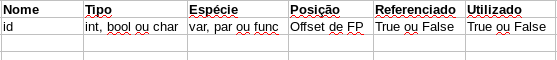
\includegraphics[scale=.75]{tabela_simbolos}
    \end{figure}

    Como dito em uma seção anterior, o compilador Allegri traduz o código diretamente a partir da sintaxe do programa. Isso significa que a cada transição entre estados, chamada ou retorno de sub-máquinas, uma rotina semântica pode ser acionada de modo a o Analisador Semântico atualizar as suas estruturas de dados e o Gerador de Código acrescentar novas instruções ao corpo do código objeto, conforme for possível.

    \subsection*{Organização da Memória}
    \addcontentsline{toc}{subsection}{Organização da Memória}
    A organização de memória de um programa determina
    \begin{itemize}
        \item sua capacidade de ter código reentrante;
        \item possibilidade de ter chamadas recursivas;
        \item o isolamento entre segmentos de código (mais proteção contra ações indevidas que prejudicam o código), etc.
    \end{itemize}

    O compilador Allegri estrutura o programa gerado em quatro segmentos. O primeiro é o de texto, onde constantes e variáveis globais são armazenados. O segundo é o segmento de código. Nele estão contidas tanto as sub-rotinas compiladas quanto o código linkado das sub-rotinas da biblioteca, as quais formam um ambiente de execução para a MVN. O terceiro é caracterizado por ter uma área que pode ser utilizada para guardar objetos de diferentes tipos e tamanhos tais como structs, vetores, matrizes, etc\footnote{Obs: por não fazer parte do escopo deste presente projeto, não foram incluídas sub-rotinas de \textit{garbage collection}}. A quarta região talvez seja a mais interessante\textemdash a Pilha. Nela são armazenados os parâmetros reais passados a funções e variáveis locais. Nela são executadas as expressões aritméticas e booleanas (ou seja, serve como área de rascunho). É o uso da pilha que permite ao código compilado ser recursivo.

    \begin{figure}[h]
        \centering
        \caption{Organização da Memória}
        \label{fig:OrgMem}
        \includegraphics[scale=0.65]{OrganizacaoMemoria}
    \end{figure}

    A figura \ref{fig:OrgMem} ilustra o modo de organização da memória da MVN.
    Note que a Pilha cresce para baixo (endereços menores), enquanto que a Heap cresce para cima. Um programa pode ter problemas com a colisão entre essas duas áreas. Porém, não foi o objetivo deste projeto gerenciar esse problema, apenas ilustrar a possibilidade de uso dessa configuração de memória.

    \subsection*{Declaração de Função}
    \addcontentsline{toc}{subsection}{Declaração de Função}

    A declaração de função consiste, basicamente, em abrí-la com uma label do tipo
    \begin{lstlisting}[frame=none,numbers=none]
    ID_FUNC        $   =1
    \end{lstlisting}
    e fechá-la com uma outra instrução do tipo
    \begin{lstlisting}[frame=none,numbers=none]
    FIM_ID_FUNC    RS  ID_FUNC
    \end{lstlisting}

    A tradução do corpo da função fica a cargo da sub-máquina Bloco.

    As declarações de parâmetros não geram código imediatamente. Porém, é muito importante determinar qual a posição cada um irá ocupar no frame de ativação. Quando uma sub-rotina é chamada, seu argumentos são passados via pilha. Se a ordem dos parâmetros for a mesma em que eles foram declarados, suas posições estarão invertidas na pilha. Por isso, é fundamental que as posições dos parâmetros atribuídas pelo compilador sejam dadas em ordem iversa à de declaração. Assim, a ordem de passagem de parâmetro coincidirá com a da organização do frame da função.

    A figura \ref{fig:FuncSem} dá uma idéia de como uma declaração é tratada pelo compilador.


    \begin{figure}[h]
        % \centering
        \caption{Rotinas semânticas associadas à declaração de função}
        \label{fig:FuncSem}
        \includegraphics[scale=.48]{semanticas/Func}
    \end{figure}

    \subsection*{Implementação de Expressões}
    \addcontentsline{toc}{subsection}{Implementação de Expressões}
    A tradução de expressões de tipo lógico-aritméticas foi, sem dúvida, o maior desafio para a implementação deste compilador. O uso da pilha de execução facilitou em muito a geração de código.

    Basicamente, o compilador utiliza duas pilhas para realizar a gerar o código das expressões:
    \begin{itemize}
        \item Pilha de Operadores: responsável por armazenar os símbolos de operações ainda não processadas. É parecida com o conceito de pilha de operadores que há no algoritmo de \textit{shunting yard} (que transforma notação infixa em posfixa). Porém, não estamos convertendo a expressão para RPN, logo são conceitos distintos;
        \item Pilha de Identificadores: responsável por armazenar os símbolos dos operandos. Ao entrar nessa pilha, o operando espera por ter seu valor carregado e empilhado na pilha de execução. Porém, como no caso de arrays e de chamadas a funções, às vezes ele tem que aguardar outras expressões serem avaliadas (e.g., índices de um array ou parâmetros de uma função). Assim se justifica o uso de uma pilha de operandos.
    \end{itemize}

    O algoritmo de tradução é, em linhas gerais, como segue:

    \begin{lstlisting}
    S = []; pilha de operandos
    T = []; pilha de operadores
    enquanto Evento != Expressoes.pop() faca
        se Evento == chegada operando entao
            S.push(operando)
            se T nao vazia e T.topo != ( entao
                operador = T.pop()
                codigo.append('SC operador')
        senao se Evento == chegada operador entao
            T.push(operador)
        fim se
    fim enquanto
    \end{lstlisting}

    Claramente estamos omitindo detalhes do algoritmo, mas a idéia é ir empilhando operandos e ir realizando as operações sobre o topo da pilha. A abertura de parênteses faz com que uma sub-expressão seja avaliada antes que uma outra operação possa ser desempilhada. Por isso o algoritmo sempre verifica se o topo da pilha de operadores não é um abre parênteses.

    O algoritmo abstrai o conceito de operando por meio da sub-máquina Operando (daí mais uma vantagem de se ter várias sub-máquinas independentes). Isso torna o parsing mais lento, mas a implementação das rotinas semânticas tornam-se muito mais genéricas. Poderiamos facilmente estender a linguagem para suportar operações com structs e objetos apenas modificando a sub-máquina Operando, por exemplo.

    A figura \ref{fig:ExpSem} dá uma idéia gráfica de como o código assembly se pareceria no final.

    \begin{figure}[h]
        \centering
        \caption{Rotinas semânticas associadas à sub-máquina Expressão}
        \label{fig:ExpSem}
        \includegraphics[scale=.75]{semanticas/exp}
    \end{figure}

    \subsection*{Chamada de Sub-rotina e Recursão}
    \addcontentsline{toc}{subsection}{Chamada de Sub-rotina e Recursão}
    Uma sob-rotina pode ser chamada ou dentro de uma expressão ou como um comando simples. Em ambos os casos, o contexto deve ser mudado desde a função chamadora (que vamos chamar de func 1) para a função chamada (func 2) e, após o retorno desta, o contexto deve ser restaurado de modo que tudo fique igual ao que estava antes para func 1, com exceção de um valor de retorno empilhado como resultado da chamada de func 2. 

    A figura \ref{fig:rotinachamadafuncao} ilustra como ocorre essa mudança de contexto.

    \begin{figure}[h]
        \centering
        \caption{Rotinas semânticas para chamada de sub-rotina}
        \label{fig:rotinachamadafuncao}
        \includegraphics[scale=.65]{semanticas/Operando_semantica}
    \end{figure}

    Já a figura \ref{fig:Frames} ilustra    a divisão da pilha em regiões de ativação entre duas funções. Ela também ilustra como deve ocorrer a divisão de responsabilidades na construção do novo frame de func 2.

    \begin{figure}[h]
        \centering
        \caption{Troca de Contexto por Frames de Ativação}
        \label{fig:Frames}
        \includegraphics[scale=.65]{Frames}
    \end{figure}


    %%%%%%%%%%%%%%%%%%%%%%%
    %      SIMULAÇÕES     %
    %%%%%%%%%%%%%%%%%%%%%%%

    \part*{Testes e Simulações\\\textit{Scherzo}}
    \addcontentsline{toc}{part}{Testes e Simulações - Scherzo}
    Passamos agora a demonstrar o uso da linguagem Barber em diversos exemplos.
    
    \subsection*{Chamada de Sub-rotina}
    \addcontentsline{toc}{section}{Chamada de Sub-rotina}
    Temos duas funções:
    \begin{itemize}
        \item f(int, int) -> int : retorna (p1+7)*(p2+2)
        \item main() -> None : sub-rotina que chama f(10, 20)
    \end{itemize}
    O objetivo deste exemplo é o de demonstrar como funciona o mecanismo de passagem de parâmetros e retorno de valor via pilha de execução.

    Código:
    \begin{lstlisting}
    def f int 
        par p1, p2 int {
        var v3, v4 int

        v4 = 2
        v3 = 7

        return (p1 + v3) * (p2 + v4)
        }

    def main {
        f(10, 20)
        }
    \end{lstlisting}
    Resultado da execução na MVN:
    \begin{figure}[h]
        \centering
        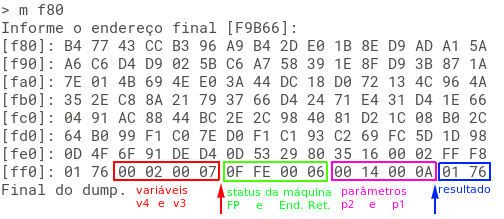
\includegraphics[scale=0.65]{chamada_subrotina}
    \end{figure}

    O dump acima revela como o código fez o gerenciamento da pilha de execução dinâmica durante a "vida" do programa.

    A seta em azul indica a posição da memória em que se encontrava FP (ponteiro de início de frame ou activation record) antes da chamada a f (ou seja, FP da sub-rotina main).
    Conforme os valores reais dos parâmetros formais vão sendo calculados, aqueles vão sendo empilhados de forma a construir uma lista de passagem de parâmetros para a função f por pilha. A sub-rotina terá acesso a esses valores por meio de cálculo de endereços relativos ao seu FP. Cada parâmetro ocupa uma posição de memória com offset bem determinado em relação a FP.

    O conteúdo do retângulo verde representa o estado anterior da sub-rotina main salvo no frame, de modo que seja possível restaurar esse estado após o retorno de f e que a execução de main possa prosseguir como se nada a houvesse interrompido. Primeiramente é salvo o endereço de retorno que está armazenado na primeira posição de memória da sub-rotina main; em segudo lugar, vem o valor de FP antigo (antes de ser atualizado por f).

    A seta em vermelho indica o novo valor de FP, o qual indicará a f onde inicia-se o seu contexto. Ou seja, indica a posição de memória que separa os frames de f e main. Tudo o que estiver além desse novo FP estará sob responsabilidade de f (tais como a alocação de novas variáveis etc.) e o que estiver aquém, está sob responsabilidade de main. A função f acessa os valores dos parâmetros passados por main por meio de acesso a endereços relativos ao seu FP. Bem como armazena suas variáveis locais a partir desse endereço. O valor de retorno de f é posto o mais próximo possível do frame de main. Desse modo procedimento de retorno da sub-rotina é feito de forma mais eficiente e, além disso, o resultado "aparecerá" para main no topo de sua pilha, agilizando o acesso a esse valor.

    Por fim, percebe-se o espaço alocado por f para as suas duas variáveis locais, v3 e v4, as quais armazenam valores constantes e, por isso, como pode-se notar, não têm seus valores alterados durante a execução do programa. Todos os cálculos  são realizados na pilha, porém, sem afetar nenhum conteúdo que lá esteja salvo.
    E last but not least, não se poderia deixar de notar que a sub-rotina f faz o cálculo como o esperado (176hex = 374dec = (10+7)*(20+2)) e armazena-o onde era suposto (como a função main não possui parâmetros nem variáveis, neste caso é a primeira posição de memória da pilha). 

    \subsection*{Expressões Aritméticas com Chamadas Aninhadas a Sub-rotinas: Reentrância}
    \addcontentsline{toc}{section}{Expressões Aritméticas com Chamadas Aninhadas a Sub-rotinas: Reentrância}
    A fim de demonstar o poder que a passagem de parâmetros via pilha de execução dinâmica acrescenta à linguagem, tendo em vista que certas expressões aritméticas podem ser escritas mais concisamente expressando-se os parâmetros de uma sub-rotina em função do resultado de outra, foi escrito o seguinte programa:

    \begin{lstlisting}
    def f int
        par p1, p2 int {
        return (p1 + p2)*2
    }

    def main {
        var a, b int
        b = 4660
        a = 3 + 6*f(3 + f(1, (7 - (1 + 4))), 5)
    }
    \end{lstlisting}

    Esse pequeno programa tem como intuito mostrar o gérmen do conceito de sub-rotina reentrante. Diz-se que uma sub-rotina é reentrante se e somente se a sua área de código for estanque em relação à área de dados. Como consequência, uma mesma porção de programa pode operar sobre áreas da memória de dados distintas - tendo-se que fazer apenas  uma mudança de contexto, claro.

    As vantagens desse esquema são várias. Dentre elas:

    \begin{enumerate}
        \item Uso eficiente da memória de programa (código compartilhado);
        \item Possibilita a implementação de sub-rotinas recursivas;
        \item Maior organização e segmentação da memória do computador;
        \item Dados de uma tarefa não correm o risco de serem alterados quando da execução da mesma sub-rotina por outra tarefa concorrente.
    \end{enumerate}

    O resultado do código compilado é mostrado a seguir:

    \begin{figure}[h]
        \centering
        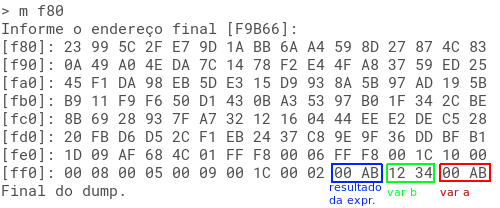
\includegraphics[scale=0.65]{chamada_subrotinas_aninhadas}
    \end{figure}

    Pode-se ver claramente que o resultado da expressão aritmética foi sendo calculado aos poucos, por meio do armazenamento de resultados parciais na pilha. Alguns deles foram sobrescritos conforme a execução do programa avançou. Porém, a ordem em que esses resultados foram calculados segue a mesma dos parâmetros de f. Por isso, f(1, (7 - (1+4))) foi calculado antes, uma vez que o seu resultado era imprescindível ao cálculo total da expresão de atribuição. Ao final, o resultado que foi colocado no topo da pilha (logo após a área das variáveis) foi corretamente atribuído a variável a (a variável b foi criada apenas para mostrar isso mais claramente).
    
    \subsection*{Fatorial: Recursividade}
    \addcontentsline{toc}{section}{Fatorial: Recursividade}
    Um dos exemplos clássicos de computação com recursão é o do cálculo do fatorial de um número. Apresento a seguir a versão desse algoritmo escrito em nossa linguagem:

    \begin{lstlisting}
    def fat int
        par n int {
        if n == 0 {
            return 1
        }
        return n * fat(n-1)
    }

    def main {
        var a, b int
        b = 6
        a = fat(b)
    }
    \end{lstlisting}

    O resultado é mostrado a seguir:
    \newpage
    \begin{figure}[h]
        \centering
        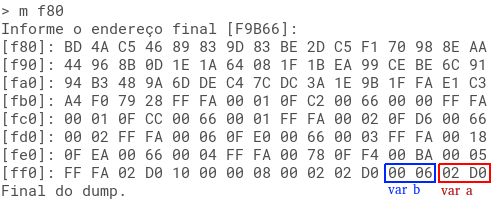
\includegraphics[scale=0.65]{fat_recursao}
    \end{figure}

    Como pode-se perceber, tal tipo de construção consome muita memória. Consumo esse causado pela grande quantidade de dados que precisam ser salvos a cada chamada da função fat.

    Nesse exemplo, calculou-se o fatorial de 6, que resulta 720dec = 2D0hex.

    Note a correta execução da condição de parada (3ª linha), quando n anula-se e tem como resultado o retorno do valor 1.
    
    \subsection*{Fatorial não recursivo}
    \addcontentsline{toc}{section}{Fatorial não recursivo}
    Esse exemplo serve apenas para demonstrar como o programa pode ficar mais enxuto e, portanto, eficiente, caso abandone-se a abordagem de chamada de funções recursivas e venha a se adotar um laço while em vez daquela. De sobra, esse exemplo demonstra o uso do tal comando while:

    \begin{lstlisting}
    def main {
        var a, b int
        a = 1
        b = 6
        while b > 0 {
            a = a * b
            b = b - 1
        }
    }
    \end{lstlisting}

    Segue o resultado:

    \begin{figure}[h]
        \centering
        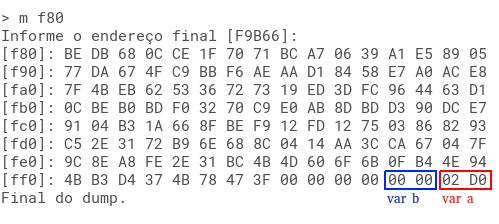
\includegraphics[scale=0.65]{fat_while}
    \end{figure}

    O resultado foi o mesmo do anterior (ufa!). Nota-se que o uso da pilha foi consideravelmente menor, o que mostra que esse programa é mais eficiente. Note o valor final da variável b. Ele coincide com o da condição de parada do loop, como era de se esperar.
    
    % \subsection*{Atribuição a Elemento de Vetor}
    % \addcontentsline{toc}{section}{Atribuição a Elemento de Vetor}
    
    \subsection*{Somatório de Elementos de Vetor}
    \addcontentsline{toc}{section}{Somatório de Elements de Vetor}

    A seguir, mostramos como a passagem de vetores e matrizes por referência pode ser útil. Definimos uma função que, dado um certo vetor v de comprimento arbitrário, retorna o somatório dos elementos de v.

    \begin{lstlisting}
    def somar int
        par v int[] {
        var i int
        var soma int

        soma = 0
        
        i = 0
        while i < len(v) {
            soma = soma + v[i]
            i = i + 1
        }
        
        return soma
    }

    def main {
        var z int[10]
        var soma, i int
        var x int
        
        i = 0
        while i < len(z) {
            z[i] = 2*i + 1
            i = i + 1
        }
        
        soma = somar(z)
        x = soma*2 + 1
    }
    \end{lstlisting}

    A seguir, o resultado da execução:

    \begin{figure}[h]
        \centering
        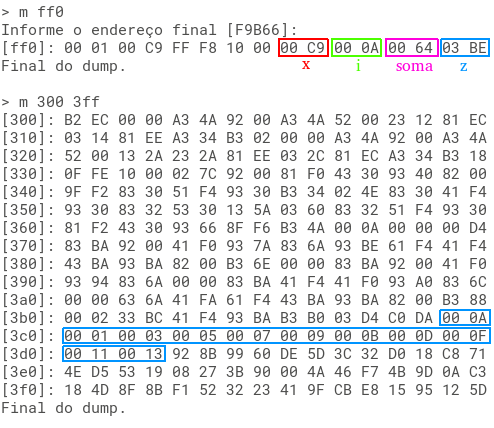
\includegraphics[scale=0.7]{soma_vetor}
    \end{figure}

    Note que não foi preciso passar como parâmetro o comprimento de v (como teríamos que fazê-lo em outras linguagens, como C e C++).

    \newpage
    \subsection*{Multiplicação de Matrizes}
    \addcontentsline{toc}{section}{Multiplicação de Matrizes}
    E, \textit{last but not least}, eis o exemplo de como pode ser implementada a função de multiplicação de matrizes em Barber.

    \begin{lstlisting}
    def mult
        par m1, m2, mr int[][] {
        var i, j, k, temp int

        i = 0
        while i < 2 {
            j = 0
            while j < 1 {
                k = 0
                temp = 0
                while k < 2 {
                    temp = temp + m1[i, k]*m2[k, j]
                    k = k + 1
                }
                mr[i, j] = temp
                j = j + 1
            }
            i = i + 1
        }

    }

    def main {
        var x int[2][2]
        var y, z int[2][1]

        x[0, 0] = 11
        x[0, 1] = 1
        x[1, 0] = 12
        x[1, 1] = 8

        y[0, 0] = 14
        y[1, 0] = 5

        mult(x, y, z)

    }
    \end{lstlisting}

    Eis o resultado da multiplicação. O que está destacado em vermelho é a matriz x 2x2; em verde, o vetor y 2x1; em azul, o vetor z 2x1.
    É mostrado, na figura abaixo, no frame da função \verb|main| os seus respectivos ponteiros para a área de dados.
    Pode-se notar claramente como os ponteiros foram passados como parâmetro para a função \verb|mult|.
    Vê-se que o resultado foi calculado corretamente e guardado no vetor z.

    \begin{figure}[h]
        \centering
        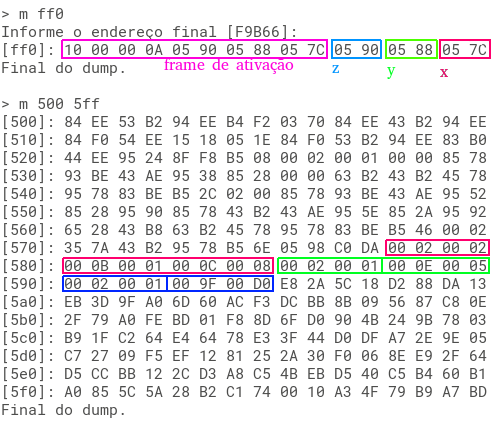
\includegraphics[scale=0.65]{mult}
    \end{figure}

    \chapter*{Finale}
    \addcontentsline{toc}{part}{Finale}
    O desenvolvimento de um compilador é, sem dúvida nenhuma, umas das tarefas mais complexas e desafiantes na área da Computação. A oportunidade de desenvolver um, ainda que didático, resultou em grande aprendizado e experiência com técnicas de análise e tradução de linguagens.

    Pessoalmente, sempre tive curiosidade de saber como os programas e as estruturas de dados eram mapeadas desde uma linguagem de alto nível para uma de baixo nível. Embora a máquina escolhida (MVN) seja bem precária em termos de conjunto de instruções, verdade seja dita, valeu a pena implementar uma linguagem Go-like para ela. Tive a oportunidade de pesquisar na Teoria quais as técnicas usuais para implementar chamadas recursivas, passagem de parâmetro por valor e referência, como gerenciar memória etc., e além disso, tive a oportunidade de adaptar aquelas soluções da literatura para uma máquina específica. Aprendi muito.
\end{document}
